\documentclass[11pt]{llncs}
%%%%%%%%%%%%%%%%%%%%%%%%%%%%%%%%%%%%%%%%%%%%%%%%%%%%%%%%%%%
%% package sillabazione italiana e uso lettere accentate
\usepackage[latin1]{inputenc}
\usepackage[english]{babel}
\usepackage[T1]{fontenc}
%%%%%%%%%%%%%%%%%%%%%%%%%%%%%%%%%%%%%%%%%%%%%%%%%%%%%%%%%%%%%

\usepackage{verbatim}
\usepackage{url}
\usepackage{xspace}
\usepackage{float}
\usepackage{url}
\usepackage{listings}
\usepackage{enumerate}

\lstdefinelanguage{contact}{
  morekeywords={ContactSystem, Context, BehaviorOf, support=, TCP, 
  state, initial, endstate, transitToEnd, goToState, onMessage, showMsg, action, var, val,
  transitTo, code., const., set, exec, call,
  doOut, doIn, doInOut, doOutIn,
  Dispatch, serve, accept,   Request, demand, grant,    Signal, emit, sense,
  Invitation, forward, to, ask,
  Subject, class, inherits, context, 
  if, null, String, Object, double, Double, Int, int, inheritedhavior},
    alsoletter={-},
  otherkeywords={=>,<-,<\%,<:,>:,\#,@},
  sensitive=true,
  morecomment=[l]{//},
  morecomment=[n]{/*}{*/},
  morestring=[b]",
  morestring=[b]',
  morestring=[b]"""
}
\usepackage{courier}
\usepackage{color}
\definecolor{dkgreen}{rgb}{0,0.6,0}
\definecolor{gray}{rgb}{0.5,0.5,0.5}
\definecolor{mauve}{rgb}{0.58,0,0.82}

\makeatletter
%%%%%%%%%%%%%%%%%%%%%%%%%%%%%% User specified LaTeX commands.
\usepackage{manifest}

\makeatother

\usepackage{ifpdf} 

\usepackage[a4paper,top=2cm,bottom=2cm,left=2cm,right=2cm]{geometry}

%%%%%%%
 \newif\ifpdf
 \ifx\pdfoutput\undefined
 \pdffalse % we are not running PDFLaTeX
 \else
 \pdfoutput=1 % we are running PDFLaTeX
 \pdftrue
 \fi
%%%%%%%
 \ifpdf
 \usepackage[pdftex]{graphicx}
 \else
 \usepackage{graphicx}
 \fi
%%%%%%%%%%%%%%%
 \ifpdf
 \DeclareGraphicsExtensions{.pdf, .jpg, .tif}
 \else
 \DeclareGraphicsExtensions{.eps, .jpg}
 \fi
%%%%%%%%%%%%%%%

\newcommand{\java}{\textsf{Java}}
\newcommand{\contact}{\emph{Contact}}
\newcommand{\corecl}{\texttt{corecl}}
\newcommand{\medcl}{\texttt{medcl}}
\newcommand{\msgcl}{\texttt{msgcl}}
\newcommand{\android}{\texttt{Android}}
\newcommand{\dsl}{\texttt{DSL}}
\newcommand{\jazz}{\texttt{Jazz}}
\newcommand{\rtc}{\texttt{RTC}}
\newcommand{\ide}{\texttt{Contact-ide}}
\newcommand{\xtext}{\texttt{XText}}
\newcommand{\xpand}{\texttt{Xpand}}
\newcommand{\xtend}{\texttt{Xtend}}
\newcommand{\pojo}{\texttt{POJO}}
\newcommand{\junit}{\texttt{JUnit}}

\newcommand{\action}[1]{\texttt{#1}\xspace}
\newcommand{\code}[1]{{\small{\texttt{#1}}}\xspace}
\newcommand{\codescript}[1]{{\scriptsize{\texttt{#1}}}\xspace}

% Cross-referencing
\newcommand{\labelsec}[1]{\label{sec:#1}}
\newcommand{\xs}[1]{\sectionname~\ref{sec:#1}}
\newcommand{\xsp}[1]{\sectionname~\ref{sec:#1} \onpagename~\pageref{sec:#1}}
\newcommand{\labelssec}[1]{\label{ssec:#1}}
\newcommand{\xss}[1]{\subsectionname~\ref{ssec:#1}}
\newcommand{\xssp}[1]{\subsectionname~\ref{ssec:#1} \onpagename~\pageref{ssec:#1}}
\newcommand{\labelsssec}[1]{\label{sssec:#1}}
\newcommand{\xsss}[1]{\subsectionname~\ref{sssec:#1}}
\newcommand{\xsssp}[1]{\subsectionname~\ref{sssec:#1} \onpagename~\pageref{sssec:#1}}
\newcommand{\labelfig}[1]{\label{fig:#1}}
\newcommand{\xf}[1]{\figurename~\ref{fig:#1}}
\newcommand{\xfp}[1]{\figurename~\ref{fig:#1} \onpagename~\pageref{fig:#1}}
\newcommand{\labeltab}[1]{\label{tab:#1}}
\newcommand{\xt}[1]{\tablename~\ref{tab:#1}}
\newcommand{\xtp}[1]{\tablename~\ref{tab:#1} \onpagename~\pageref{tab:#1}}
% Category Names
\newcommand{\sectionname}{Section}
\newcommand{\subsectionname}{Subsection}
\newcommand{\sectionsname}{Sections}
\newcommand{\subsectionsname}{Subsections}
\newcommand{\secname}{\sectionname}
\newcommand{\ssecname}{\subsectionname}
\newcommand{\secsname}{\sectionsname}
\newcommand{\ssecsname}{\subsectionsname}
\newcommand{\onpagename}{on page}

\newcommand{\xauthA}{Roberto Casadei}
\newcommand{\xauthB}{}
\newcommand{\xauthC}{}
\newcommand{\xfaculty}{Ingegneria e Scienze Informatiche}
\newcommand{\xunibo}{Alma Mater Studiorum -- University of Bologna}
\newcommand{\xaddrBO}{viale Risorgimento 2}
\newcommand{\xaddrCE}{via Venezia 52}
\newcommand{\xcityBO}{40136 Bologna, Italy}
\newcommand{\xcityCE}{47023 Cesena, Italy}

%
% Comments
%
%%% \newcommand{\todo}[1]{\bf{TODO:}\emph{#1}}

\usepackage{listings}

\usepackage{amssymb}
\renewcommand{\labelitemi}{\tiny$\blacksquare$}
\begin{document}

\title{Semantic Web: from Relational DataBase to Ontology}

%%% \author{\xauthA \and \xauthB}
\author{\xauthA\\roberto.casadei12@studio.unibo.it}

\institute{%
%%%  \xunibo\\\xaddrCE, \xcityCE\\\email{\{nameA.studentA, nameB.studentB\}@studio.unibo.it}
  \xunibo\\ Master's Degree in Computer science and Engineering \\ \emph{Within the Semantic Web course}\\
}

\maketitle


%% \begin{abstract}
%% \footnotesize
%%This a Latex template to be used for the reports of Software Engineering.
%%\keywords{Software engineering, managed software development, reports, ....}
%%\end{abstract}

%%% \sloppy

%===========================================================================
\section{Introduction}
\labelsec{intro}
%===========================================================================

This report describes my final work and research within the course ``Semantic Web''.$\\$
The previous assignments were about
\begin{enumerate}
 \item introducing the topic of the Semantic Web as well as providing some insights about its spread in the industry
 \item modelling a domain of interest and developing a (weak) ontology using RDF Schema
 \item modelling a domain of interest and developing a (strong) ontology using OWL
\end{enumerate}
where I chose the ``Project Management'' domain as the object of my modelling efforts.$\\$

This final work is still about the development of an ontology, but the information to be used is (assumed to be already) provided by a 
 Relational DataBase (RDB). 
 In other words, the general problem to be faced is: \emph{how can we convert relational data into RDF/OWL form}? $\\$
 My goal is twofold:
 \begin{enumerate}
  \item look at the state-of-art of the problem
  \item turn the result of such research into action by performing an RDB-to-RDF conversion of a sample database.
 \end{enumerate}
 
%===========================================================================
\section{Basics: Relational DataBases and the Semantic Web}
\labelsec{rdbsAndSW}
%===========================================================================
 
First of all, a natural question may arise: 
\textbf{\emph{why should we care about the mapping between relational databases and RDF}}?$\\$
 The Semantic Web is not a revolution, but a gradual process, a shift towards a Web of Data where information can be
  more easily accessed, discovered, integrated, and used by both machines and humans. It is conceived as an extension,
  rather than a replacement, to the ``Syntactic Web'' where existing tools are reused when possible.$\\$
 Now, it turns out that, while NoSQL systems and triple stores are increasingly adopted (see Figure \ref{fig:dbtrend}), 
 \textbf{Relational DBMSs still dominate the database market} (see Figure \ref{fig:dbproportion}). 
 Moreover, if we just consider the Web part of the global data space, 
 because \textbf{the majority of dynamic Web content is backed by RDBs} \cite{Ravi2009}, 
 it is clear that the ability to leverage on these data is critical for the success 
  of the Semantic Web.
  

 \begin{figure}[H]
\centering
 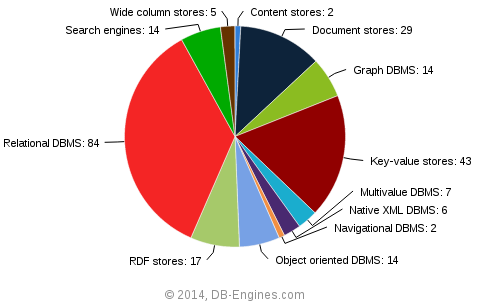
\includegraphics[scale = 0.6]{img/dbprop.png}
  \caption{Number of systems per category, June 2014}
 \label{fig:dbproportion}
\end{figure} 


 \begin{figure}[H]
 \centering
 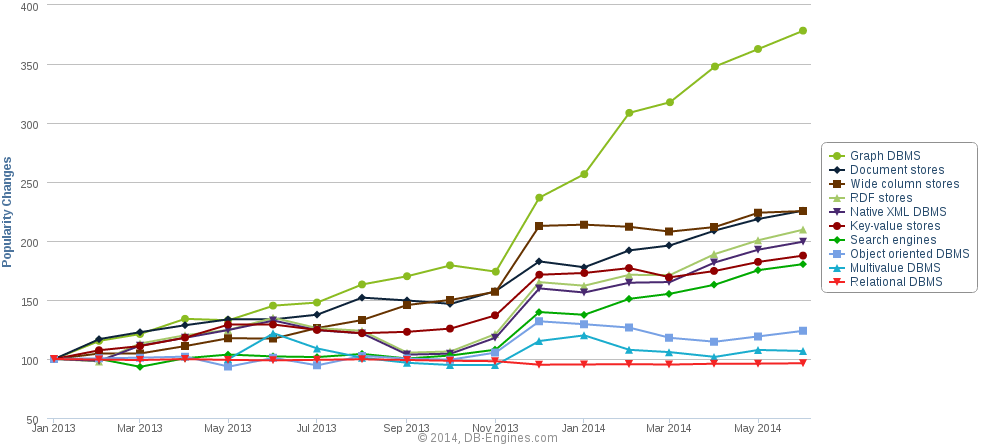
\includegraphics[scale = 0.5]{img/dbtrend.png}
  \caption{Popularity changes per category, June 2014}
 \label{fig:dbtrend}
\end{figure}

The Semantic Web is the Web of Data and data is everywhere, with relational databases being a widespread container.
 Thus, \textbf{the challenge is to export these data into a common format so to enable them 
 for interoperability within the Semantic Web ecosystem. Such a common format is RDF} (see Figure \ref{fig:swstack}).

 \begin{figure}[H]
 \centering
 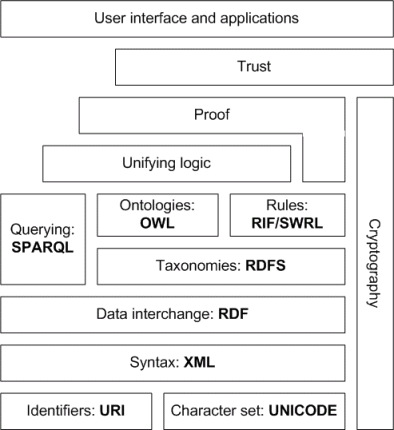
\includegraphics[scale = 0.5]{img/swstack.png}
  \caption{The Semantic Web stack}
 \label{fig:swstack}
\end{figure}  

It should also be noted that such an interaction between the Semantic Web community and the database community 
 does represent an attractive opportunity for the latter as well, where distribution, integration, and deduction
 are significant issues.$\\$
 
In a nutshell, the main motivations and opportunities arising 
from bringing relational databases in the Semantic Web \cite{bringingRDBS} are the following:
\begin{itemize}
 \item \emph{Integration of RDBs with other data sources} (see above)
 \item \emph{Generation of a critical mass of data for the Semantic Web}: 
 by automatic extraction of information from RDBs into RDF (see above)
 \item \emph{Heterogeneous database integration}: with ontology-based integration as an alternative to an integration approach
  based on conceptual models
 \item \emph{Semantic annotation of dynamic (RDB-backed) web pages}: augmenting web content with semantic labels 
  which are generated based on the mappings between the RDB schema and existing ontologies
 \item \emph{Ontology-based data access of the RDB}: allowing users to write semantic queries which are rewritten into SQL
 \item \emph{Ontology learning}: as ontology development is not an easy task, exploiting the information of an RDB (not just 
  schema and data but also metadata, queries, views, stored procedures) to derive an ontology which can be subsequently 
  extended/refined is alluring
 \item \emph{Specification of the semantics of relational schemas}: as an alternative to maintaining and  keeping aligned 
  the original conceptual model with the relational schema, defining a mapping between the schema and an ontology
  provides meaning for designers and provides support for DB maintainance and integration as well as representing 
  a common model for database reconciliation
\end{itemize}

%Here, in particular, the focus is on the mapping between RDBs (where data is represented in the relational model) and RDF graphs 
% (where data is represented in the RDF data model).
% ???? Mapping at data-level or schema-level

%===========================================================================
\subsection{Converting relational data into RDF data}
\labelsec{rdfDataManagement}
%===========================================================================

In general, relational data can be made available in RDF form using two approaches (see Figure \ref{fig:rdfmanagement}).
One approach consists in performing a \emph{physical} conversion (aka \emph{RDF dump}), where 
 relational data is \textbf{extracted, transformed, and loaded (ETL)} into a triple store which represents the 
 \textbf{\emph{materialized} view} of the original RDB.
The other approach works by providing a \textbf{\emph{virtual} view} of the relational database as a RDF graph. 
 In this case, for example, SPARQL queries can be translated into equivalent SQL queries which are then issued against the RDB.

 \begin{figure}[H]
 \centering
 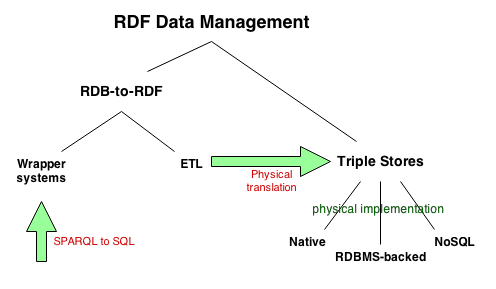
\includegraphics[scale = 0.6]{img/rdfmanagement.png}
  \caption{RDF Data Management and Relational Databases \cite{rdb2rdf_vimeo_euclid}}
 \label{fig:rdfmanagement}
\end{figure}  

The creation of an RDF view of relational data allows them to become part of the Web of Data (see Figure \ref{fig:rdb2rdf_principle}),
 thus inheriting significant advantages in terms of access and data integration which make them unleash their value.
 For example, a typical use case consists in the need of integrating an RDB 
 with other data represented in a different form using RDF as a medium.

 \begin{figure}[H]
 \centering
 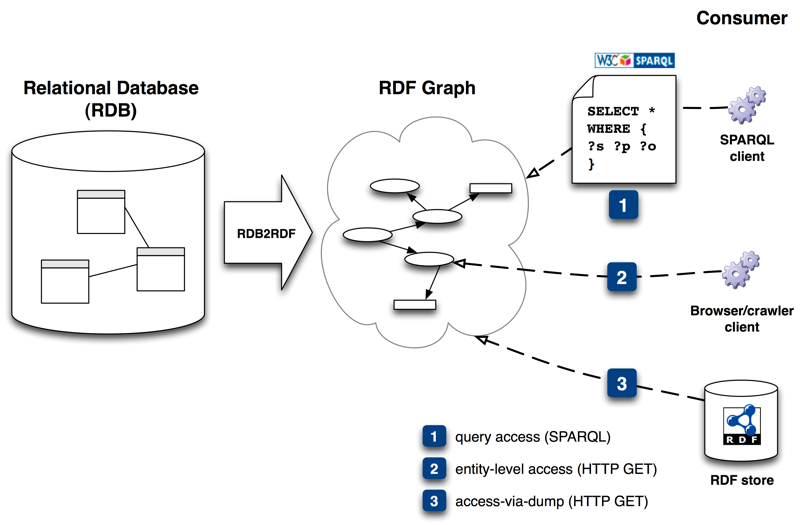
\includegraphics[scale = 1.6]{img/rdb2rdf_principle.png}
  \caption{On the RDF view of a relational database many kinds of access are supported. \cite{W3UCMapping}}
 \label{fig:rdb2rdf_principle}
\end{figure}

%===========================================================================
\section{Mapping between the Relational Model and the RDF Model}
\labelsec{mapping}
%===========================================================================

It should be noted that the RDB-to-RDF transformation process happens at two levels or stages:
\begin{enumerate}
 \item at the \emph{intension}-level: where the relational schema is put in relation with a projected or an existing/custom ontology, and
 \item at the \emph{extension}-level: where the instances of the relational DB are converted into an RDF graph using the mappings
\end{enumerate}

So, the challenge is to \textbf{how to produce the mappings}.$\\$
The approach to mapping generation can be
\begin{itemize}
 \item \emph{Automatic}: where the mappings are automatically generated given the relational schema (and, if possible/needed, 
 some destination ontologies)
  (see Figure \ref{fig:mapping_auto})
 \item \emph{Semi-automatic}: where some mappings are automatically generated but need to be extended or refined by the user
  (see Figure \ref{fig:mapping_semi})
 \item \emph{Manual}: where the user defines the mappings by hand using a RDB-to-RDF mapping language or a tool
  (see Figure \ref{fig:mapping_manual})
\end{itemize}


\begin{figure}[!htb]
\minipage{0.32\textwidth}
 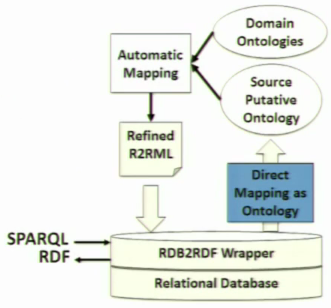
\includegraphics[scale = 0.35]{img/automaticMapping.png}
  \caption{Automatic mapping. \cite{rdb2rdf_vimeo_euclid}}
  \label{fig:mapping_auto}
\endminipage\hfill
\minipage{0.32\textwidth}
 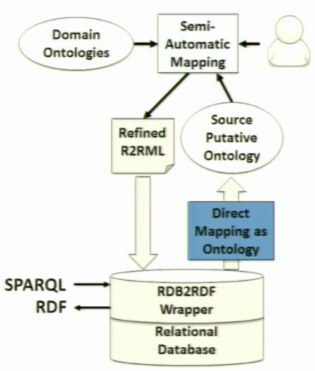
\includegraphics[scale = 0.35]{img/semiautomaticMapping.png}
  \caption{Semiautomatic mapping. \cite{rdb2rdf_vimeo_euclid}}
  \label{fig:mapping_semi}
\endminipage\hfill
\minipage{0.32\textwidth}%
 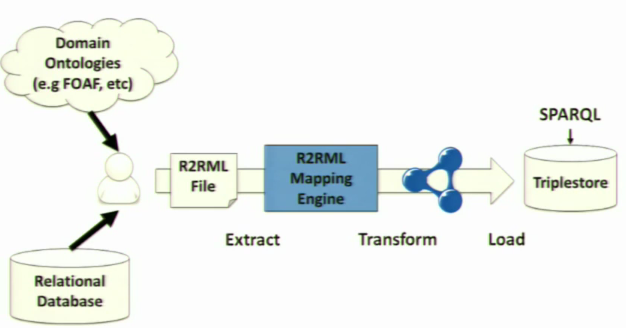
\includegraphics[scale = 0.3]{img/manualMapping.png}
 \caption{Manual mapping. \cite{rdb2rdf_vimeo_euclid}}
 \label{fig:mapping_manual}
\endminipage
\end{figure}

Typically, as ontology languages such as OWL are more expressive then the relational model, 
 the automatically generated mappings are not sufficient to capture a desired level of domain semantics.
However, they provide a basis for subsequent refinements.
Moreover, rather than simply generating an ontological projection of the relational schema, some existing
 ontology can be used to improve the quality of mappings or to guide to process within well-defined ontological boundaries.
Anyhow, when applications require complex domain semantics to be expressed, 
 the semi-automatic/manual approaches are much probably necessary. 
 
% Approaches to mapping generation
% Automatic - semiautomatic - manual

%===========================================================================
\subsection{W3C RDB2RDF activities}
\labelsec{w3activity}
%===========================================================================
In 2008, the RDB2RDF Incubator Group was launched by the W3C with the mission to

\begin{quote}
 \textit{``
to \textbf{examine and classify existing approaches} to mapping relational data into RDF and 
assess whether standardization is possible and/or necessary in this area''}
\end{quote}

The survey \cite{w3survey} inspected many projects (prototypes, domain-specific projects, and existing tools) 
 and was carried out by considering the following elements: 
\begin{itemize}
 \item \emph{Creation of mappings}: the approaches are classified in two broad classes
 \begin{enumerate}[(a)]
  \item \textbf{Automatic mapping} (aka \textbf{local ontology mapping}): where the starting point is the relational schema
  \item \textbf{Domain semantics-driven mapping} (aka \textbf{domain ontology mapping}): 
   there is some destination ontology to be populated;
   usually more precise (also useful for reducing the size of the resulting RDF graph) as more domain semantics is provided
 \end{enumerate}
 
 \item \emph{Mapping representation and accessibility}: this dimension evaluates the languages used to express the mappings
 
  \item \emph{Mapping implementation}: where two implementation strategies 
  -- \textbf{ETL-based (static)} and \textbf{query-based (dynamic)} -- are considered
 
 \item \emph{Query implementation}: where two possibilities are found: \textbf{SPARQL} queries on the resulting RDF repository
    and SPARQL queries translated to SQL queries (\textbf{SPARQL-to-SQL}) on the original RDB 
 
 \item \emph{Application domain}: the approaches to (and the tools for) mapping generation can be \textbf{generic}
 or \textbf{domain-specific}
 
 \item \emph{Data integration}: this dimension considers the different mapping methods with respect to data integration
 
\end{itemize}

One of the conclusions of such a survey is the assessment of the \textbf{need of a standard language} 
 for the representation of RDB-to-RDF mappings. The reason is essentially to allow for the \textbf{reuse} of the mappings
 across different databases and RDBMSs.$\\$

With such an input, in 2009, the W3C started an RDB2RDF Working group.

\begin{quote}
 \textit{``The mission of the RDB2RDF Working Group, part of the Semantic Web Activity, 
 is to \textbf{standardize languages} for mapping relational data and relational database schemas into RDF and OWL. 
 The two languages are the Direct Mapping (DM) and the RDB2RDF Mapping Language (R2RML)''}
\end{quote}

From the analysis of some use cases, a core set of requirements for the R2RML mapping language were proposed \cite{W3UCMapping}:
\begin{itemize}
 \item Direct mapping support (to produce a local ontology)
 \item Transformative mapping support (towards a destination ontology)
 \item Generation of globally unique identifiers
 \item Sufficient expressivity to support query translation (e.g., SPARQL to SQL)
 \item Sufficient expressivity to support ETL (RDF dump)
 \item Datatypes
    \begin{itemize}
     \item Mapping relational data types to XML Schema data types
     \item Extensibility mechanisms to support mappings for vendor-specific data types
    \end{itemize}
 \item ...Other more technical requirements...

\end{itemize}



%===========================================================================
\section{Standard RDB-to-RDF mapping languages}
\labelsec{stdmapping}
%===========================================================================

\subsection{Direct Mapping}
\labelsec{directMapping}

The direct mapping produces an RDF representation (also known as the \textbf{direct graph}) of a relational database.$\\$
The rules for the direct mapping are the following ones \cite{w3directmapping}:
\begin{itemize}
 \item \textbf{Row type triple}
 \begin{itemize}
  \item Subject: \emph{row node}
  \item Predicate: \emph{rdf:type} 
  \item Object: \emph{table resource}
 \end{itemize}
 
 \item \textbf{Literal triple}
 \begin{itemize}
  \item Subject: \emph{row node} 
  \item Predicate: \emph{column resource}
  \item Object: \emph{literal value}
 \end{itemize}
 
 \item \textbf{Reference triple}
 \begin{itemize}
  \item Subject: \emph{row node}
  \item Predicate: \emph{foreign key column resource}
  \item Object: \emph{(referenced-)row node}
 \end{itemize} 
\end{itemize}

The identifiers are created using the following schema:
\begin{itemize}
 \item Row node: <\textbf{BaseIRI/DB/TableName/PKAttr1=value1;PKAttr2=value2;...}>
 \begin{itemize}
  \item NOTE: if the table has no primary key, a new blank node is created
 \end{itemize}
 
 \item Table resource: <\textbf{BaseIRI/DB/TableName}>
 \item Column resource: <\textbf{BaseIRI/DB/TableName\#ColumnName}>
 \item Foreign key column resource: <\textbf{BaseIRI/DB/TableName\#ref-FKColumn1;FKColumn2;...}>
\end{itemize}

Note how relative IRIs are concatenated to a base IRI in order to support the uniqueness of identifiers.$\\$

The direct mapping suffers of some limitations. For example, as the direct graph reflects the structure and the names 
of the relational schema, if the schema is particularly complex or not normalized, the result may be poor.
 Similarly, the IRIs may NOT be user-friendly. Moreover, the relational schema is NOT mapped into an OWL ontology.


\subsection{RDB to RDF Mapping Language (R2RML)}
\labelsec{r2rml}

R2RML \cite{w3r2rml} is a standard language for defining mappings to transform an RDB into RDF.
 An R2RML mapping is itself represented as RDF.


\begin{figure}[H]
 \centering
 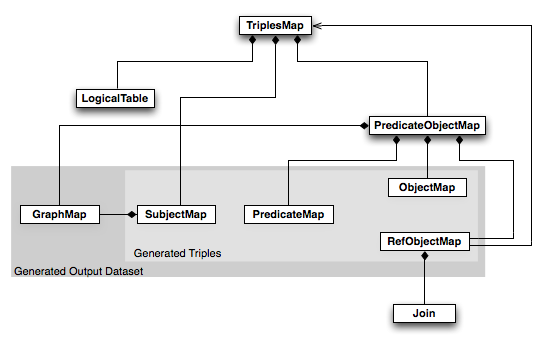
\includegraphics[scale = 0.6]{img/r2rml-overview.png}
 \caption{R2RML overview}
 \label{fig:r2rml}
\end{figure}

R2RML works by mapping \textbf{triples maps} to logical tables. A \textbf{logical table} is a table, a view, or a SQL query 
 (aka R2RML view). A triple map creates a correspondence between a table row and a set of RDF triples.
 A triple map is composed of subject maps, predicate maps, and object maps.
 The \textbf{output dataset} consists of a default (unnamed) graph and possibly more (IRI-)named graphs. 
  The generated triples can be assigned to one or more of these graphs.

  
  
%===========================================================================
\section{From Relational DataBase to Ontology}
\labelsec{r2owl}
%===========================================================================  
 
 Many of the things we would like to do with a relational database (see opportunities and motivations in Section \ref{sec:rdbsAndSW})
  are not limited to the generation of an RDF representation of the RDB content but also need to deal with 
  semantics at higher levels. So, the \textbf{\emph{DB to Ontology mapping problem (DB2O)}} is to be tackled.$\\$
 This problem has been referred to when considering the following distinct but closely related issues \cite{bringingRDBS}:
\begin{enumerate}
 \item Generation of a brand-new ontology from an RDB 
 \item Generating an RDF graph which reflects the content of an RDB 
  where RDF statements are annotated in terms of existing ontologies 
  (problem essentially solved by the R2RML standard, see Section \ref{sec:mapping})
 \item Performing semantic queries (e.g., SPARQL queries) on an RDB	
 \item Discovering the mappings between an RDB and existing ontologies
\end{enumerate}

 \begin{figure}[H]
 \centering
 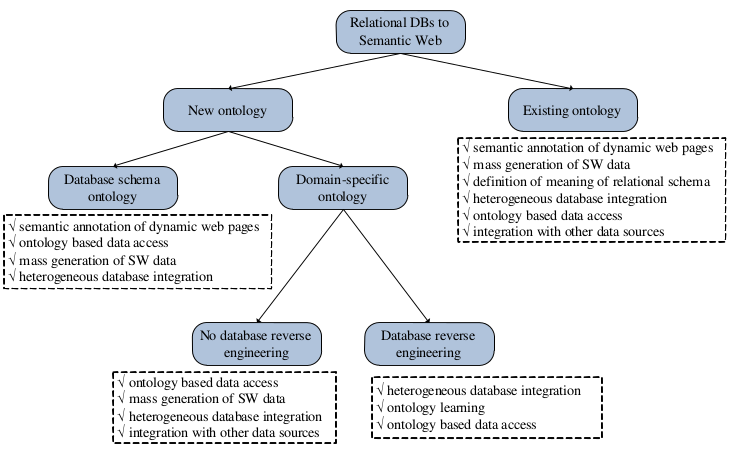
\includegraphics[scale = 0.6]{img/taxonomyApproaches.png}
 \caption{A total, exclusive classification of RDB-to-SW approaches \cite{bringingRDBS}}
 \label{fig:taxonomyApproaches}
\end{figure}

 A taxonomy of the solutions for the DB2O problem from an ontological perspective can be found in \cite{bringingRDBS}
  (see Figure \ref{fig:taxonomyApproaches}):
\begin{itemize}
 \item Level 1: ``New ontology'' vs. ``Existing ontology''
 \begin{itemize}
    \item Genus: a set of RDB-to-ontology mappings are produced
    \item Differentia: a new ontology is created vs. the mappings are defined in terms of an existing ontology
 \end{itemize}

 \item Level 2: ``DB schema ontology'' vs. ``Domain-specific ontology''
 \begin{itemize}
    \item Genus: a new ontology is generated
    \item Differentia: the new ontology directly reflects the DB schema (\emph{database schema ontology}) vs. 
     the new ontology models domain concepts
 \end{itemize} 
 
 \item Level 3: ``DB reverse engineering'' vs. ``No DB reverse engineering''
 \begin{itemize}
    \item Genus: a new domain-specific ontology is produced as output
    \item Differentia: a reverse engineering process is vs. not performed in order to extract a conceptual schema which is then 
     mapped to an ontology
 \end{itemize} 
 
\end{itemize}
  
 In general, the process of extracting an ontology from a relational database is performed by a \textbf{mapping engine} 
 (see Figure \ref{fig:rdb2ont})
  which uses a set of mappings and rules which may be written by a developer (possibly with a tool) or 
  pre-defined inside the engine.
  
 \begin{figure}[H]
 \centering
 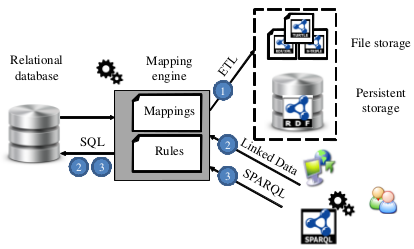
\includegraphics[scale = 0.75]{img/rdb2ontology.png}
 \caption{RDB-to-Ontology \cite{bringingRDBS}}
 \label{fig:rdb2ont}
\end{figure}  

 As you may have noted, conceptually there is no difference with respect to 
  the RDB-to-RDF process we have seen in Section \ref{sec:mapping}.$\\$
  
 In this section, the focus is on the generation of a brand-new domain-specific ontology from an RDB. 
  For the purpose, it may be useful to differentiate between two kinds of components in ontologies:
\begin{itemize}
 \item \textbf{TBox} (\textbf{T}erminological): axioms and definitions about concepts and properties
 \item \textbf{ABox} (\textbf{A}ssertion): statements about individuals
\end{itemize}
 Roughly, we would like to generate the TBox (ontology schema) from the DB's intensional knowledge 
  and the ABox (ontology instance data) from the DB's extensional knowledge as depicted in Figure \ref{fig:atbox}.

 \begin{figure}[H]
 \centering
 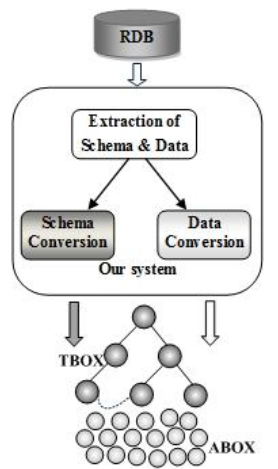
\includegraphics[scale = 0.40]{img/twoLevels.png}
 \caption{Ontology TBox and ABox generation \cite{atbox}}
 \label{fig:atbox}
\end{figure}   

However, note that not just the relational schema but also the instance data can be exploited to derive TBox statements, e.g.,
 by employing correlation analysis and data mining techniques.
  
 \subsection{A simple method}

 A basic method consists in mapping
 \begin{itemize}
  \item tables to classes
  \item rows to individuals
  \item columns to data properties
  \item foreign key columns to object properties
  \item rows' attributes to property values (or other individuals in case of reference)
 \end{itemize}
(where the OWL terminology is used).$\\$
This is sometimes called \textbf{``table-to-class, column-to-predicate''} and is somehow similar to what we have seen 
 when covering the RDB-2-RDF Direct Mapping (see Section \ref{sec:directMapping}).$\\$
 
The plain basic method presented above suffers of many drawbacks (e.g., it would create a class for many-to-many tables as well), 
however it can be extended and refined into more effective methods/tools which 
 provide some degree of support for features such as:
\begin{itemize}
 \item Mapping customization
 \item Conditional mappings
 \item DB semantics extraction mechanisms
 \item Pattern-based customization of identifiers (IRIs)
 \item Application of transformation functions to values
 \item Mapping attribute domains to classes
 \item and more
\end{itemize}


\subsection{Intermediate models}

Getting an OWL ontology from a RDB can be seen as a \textbf{Model-to-Model (M2M)} transformation.
 The impedance mismatch may result into complex mappings or operational issues. So, a simplification technique consists in
  splitting the transformation process into two or more phases. 
  Examples can be found in \cite{mappingIntoOwlStructure} (see Figure \ref{fig:intermediate}) and
  in \cite{owlxslt} (in which case the relational schema is converted into an XML Schema which is then transformed into OWL via XSLT);
   methods for transforming Entity/Relationships (E/R) models into OWL ontologies have also been explored in the literature. 

\begin{figure}[H]
 \centering
 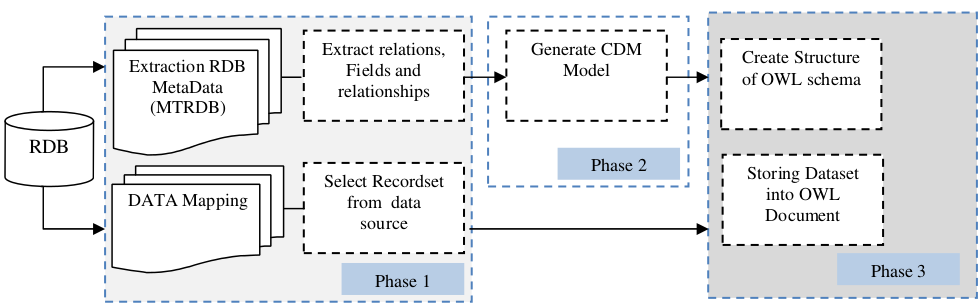
\includegraphics[scale = 0.45]{img/methodology1.png}
 \caption{A Canonical Data Model as an intermediate model.}
 \label{fig:intermediate}
\end{figure} 

 Often, these approaches make use of \textbf{heuristic rules} which looks for characteristics in the relational schema 
  in order to decide how the elements are to be treated. For example, database tables may be distinguished into
   different kinds based on the number of primary keys or foreign keys. A rough categorization of these rules 
   is provided in \cite{bringingRDBS}. The main issues are the following:
\begin{itemize}
 \item Efficiency (especially when formal methods are employed)
 \item Correctness of the inferred meaning
 \item Expressivity with respect to high-level axioms
 \item Ontology features to be generated vs. decidability of the resulting ontology
\end{itemize}
   
  Thus, sometimes the intervention of human domain experts is required 
  at certain decision points, for adjustments, or for validation.
  
  
%===========================================================================
\section{Generating an ontology from a sample ``Project Management'' DB}
\labelsec{inaction}
%===========================================================================  

The goal of this section is to illustrate how to produce an OWL ontology in the domain of project management 
 by extracting the semantics from a relational database.

\subsection{The methodology}

The process (represented as a black box in Figure \ref{fig:blackbox}) has the following inputs:
\begin{enumerate}
 \item A relational database: schema and instance data
 \item Knowledge of the target domain (project management domain)
 \item Knowledge of a target ontology language (such as OWL)
 \item Knowledge of an RDB-to-ontology mapping language (such as R2RML)
\end{enumerate}
and the output is an (OWL) ontology in the target domain.

 \begin{figure}[H]
 \centering
 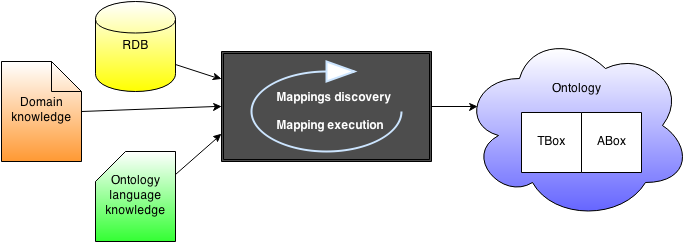
\includegraphics[scale = 0.55]{img/blackbox.png}
 \caption{The process}
 \label{fig:blackbox}
\end{figure} 

Moreover, the following steps need to be carried out:
\begin{enumerate}
 \item Preparation of the relational database: refactoring, normalization, data cleaning (SKIPPED)
 \item Analysis and development of a conceptual model or desired destination ontology (SKIPPED: THE WORK OF PREVIOUS ASSIGNMENT IS REUSED)
 \item Direct mapping generation 
 \item Refinement and enrichment of the mappings
 \item Implementation of the mapping procedure (manually or using a tool) to produce an ontology as a result
\end{enumerate}

\subsection{Inputs}
The schema and the data of the sample relational database is shown, respectively, in Figure \ref{fig:relationalSchema} and
 \ref{fig:relationalData}.

 \begin{figure}[H]
 \centering
 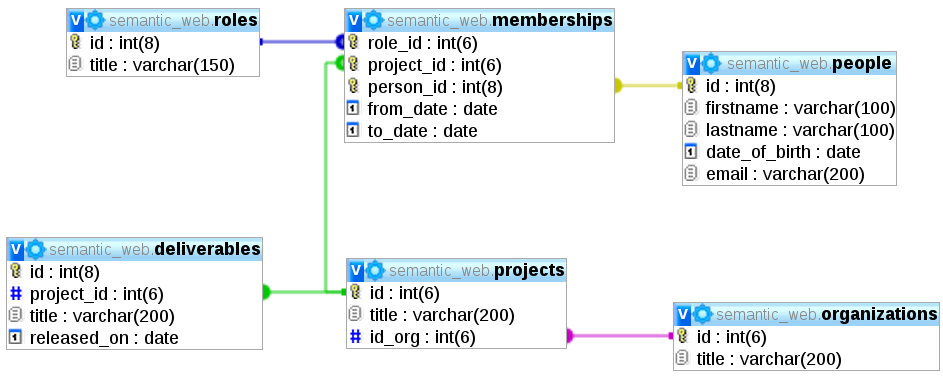
\includegraphics[scale = 0.55]{img/relationalSchema.png}
 \caption{The source schema for our examples}
 \label{fig:relationalSchema}
\end{figure} 

 \begin{figure}[H]
 \centering
 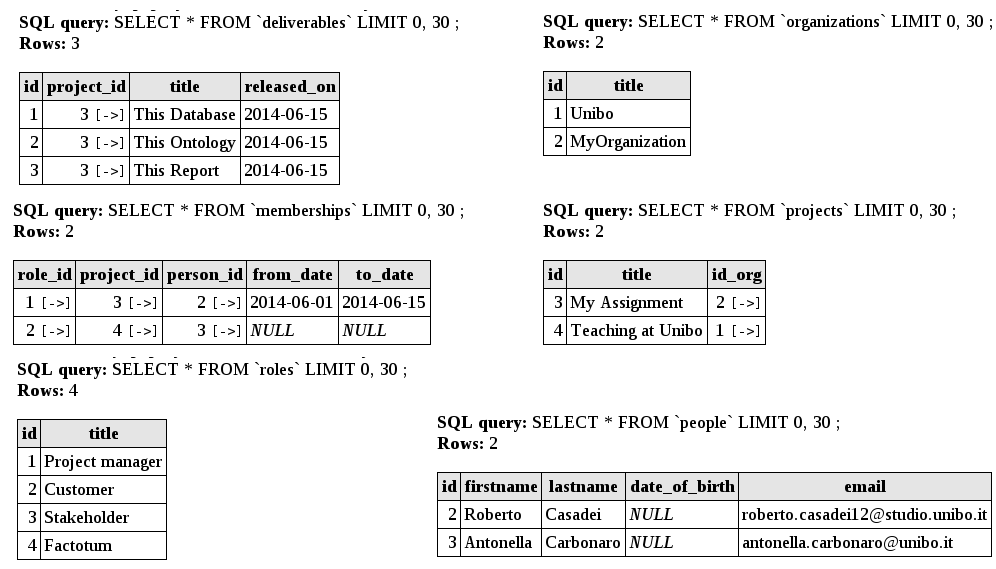
\includegraphics[scale = 0.4]{img/relationalData.png}
 \caption{The source data for our examples}
 \label{fig:relationalData}
\end{figure} 

 Note that there are two kinds of instance data. One kind is relative to ontology individuals. The other kind is 
  about project-specific data which does not belong to the ontology but to an actual project management effort.

\subsection{Direct mapping into RDFS/OWL}

For the purpose, I use the D2RQ tool\footnote{http://d2rq.org/}.

\begin{lstlisting}[language=bash]
  d2rq/$ ./generate-mapping --w3c -v -u <user> -p <pass> 
	jdbc:mysql://localhost/semantic_web
\end{lstlisting}

which produces the following output:

\lstset{basicstyle=\ttfamily\tiny, frame=single, morekeywords={a, rdfs:domain, rdfs:label, rdfs:range, rdfs:isDefinedBy, owl:DaatatypeProperty, owl:ObjectProperty, owl:Class, owl:Property}, }
\begin{lstlisting}
@prefix dc:      <http://purl.org/dc/elements/1.1/> .
@prefix :        <vocab/> .
@prefix rdfs:    <http://www.w3.org/2000/01/rdf-schema#> .
@prefix owl:     <http://www.w3.org/2002/07/owl#> .
@prefix xsd:     <http://www.w3.org/2001/XMLSchema#> .
@prefix rdf:     <http://www.w3.org/1999/02/22-rdf-syntax-ns#> .

:organizations_id
      a       rdf:Property , owl:DatatypeProperty ;
      rdfs:domain :organizations ;
      rdfs:label "organizations_id" ;
      rdfs:range xsd:integer .

:deliverables_id
      a       rdf:Property , owl:DatatypeProperty ;
      rdfs:domain :deliverables ;
      rdfs:label "deliverables_id" ;
      rdfs:range xsd:integer .

:people_firstname
      a       rdf:Property , owl:DatatypeProperty ;
      rdfs:domain :people ;
      rdfs:label "people_firstname" ;
      rdfs:range xsd:string .

:deliverables
      a       owl:Class , rdfs:Class ;
      rdfs:label "deliverables" .

:projects_id
      a       rdf:Property , owl:DatatypeProperty ;
      rdfs:domain :projects ;
      rdfs:label "projects_id" ;
      rdfs:range xsd:integer .

:projects_title
      a       rdf:Property , owl:DatatypeProperty ;
      rdfs:domain :projects ;
      rdfs:label "projects_title" ;
      rdfs:range xsd:string .

:memberships_role_id
      a       rdf:Property , owl:DatatypeProperty , owl:ObjectProperty ;
      rdfs:domain :memberships ;
      rdfs:label "memberships_role_id" ;
      rdfs:range xsd:integer , :roles .

:memberships
      a       owl:Class , rdfs:Class ;
      rdfs:label "memberships" .

:memberships_project_id
      a       rdf:Property , owl:DatatypeProperty , owl:ObjectProperty ;
      rdfs:domain :memberships ;
      rdfs:label "memberships_project_id" ;
      rdfs:range :projects , xsd:integer .

:people_lastname
      a       rdf:Property , owl:DatatypeProperty ;
      rdfs:domain :people ;
      rdfs:label "people_lastname" ;
      rdfs:range xsd:string .

:people_email
      a       rdf:Property , owl:DatatypeProperty ;
      rdfs:domain :people ;
      rdfs:label "people_email" ;
      rdfs:range xsd:string .

:people
      a       owl:Class , rdfs:Class ;
      rdfs:label "people" .

:people_id
      a       rdf:Property , owl:DatatypeProperty ;
      rdfs:domain :people ;
      rdfs:label "people_id" ;
      rdfs:range xsd:integer .

:roles_id
      a       rdf:Property , owl:DatatypeProperty ;
      rdfs:domain :roles ;
      rdfs:label "roles_id" ;
      rdfs:range xsd:integer .

:roles
      a       owl:Class , rdfs:Class ;
      rdfs:label "roles" .

:roles_title
      a       rdf:Property , owl:DatatypeProperty ;
      rdfs:domain :roles ;
      rdfs:label "roles_title" ;
      rdfs:range xsd:string .

:organizations_title
      a       rdf:Property , owl:DatatypeProperty ;
      rdfs:domain :organizations ;
      rdfs:label "organizations_title" ;
      rdfs:range xsd:string .

:organizations
      a       owl:Class , rdfs:Class ;
      rdfs:label "organizations" .

:memberships_to_date
      a       rdf:Property , owl:DatatypeProperty ;
      rdfs:domain :memberships ;
      rdfs:label "memberships_to_date" ;
      rdfs:range xsd:date .

:deliverables_released_on
      a       rdf:Property , owl:DatatypeProperty ;
      rdfs:domain :deliverables ;
      rdfs:label "deliverables_released_on" ;
      rdfs:range xsd:date .

:memberships_person_id
      a       rdf:Property , owl:DatatypeProperty , owl:ObjectProperty ;
      rdfs:domain :memberships ;
      rdfs:label "memberships_person_id" ;
      rdfs:range :people , xsd:integer .

:projects_id_org
      a       rdf:Property , owl:DatatypeProperty , owl:ObjectProperty ;
      rdfs:domain :projects ;
      rdfs:label "projects_id_org" ;
      rdfs:range :organizations , xsd:integer .

:projects
      a       owl:Class , rdfs:Class ;
      rdfs:label "projects" .

:memberships_from_date
      a       rdf:Property , owl:DatatypeProperty ;
      rdfs:domain :memberships ;
      rdfs:label "memberships_from_date" ;
      rdfs:range xsd:date .

:people_date_of_birth
      a       rdf:Property , owl:DatatypeProperty ;
      rdfs:domain :people ;
            rdfs:label "people_date_of_birth" ;
      rdfs:range xsd:date .

:deliverables_title
      a       rdf:Property , owl:DatatypeProperty ;
      rdfs:domain :deliverables ;
      rdfs:label "deliverables_title" ;
      rdfs:range xsd:string .

:deliverables_project_id
      a       rdf:Property , owl:DatatypeProperty , owl:ObjectProperty ;
      rdfs:domain :deliverables ;
      rdfs:label "deliverables_project_id" ;
      rdfs:range :projects , xsd:integer . 
\end{lstlisting}


\subsection{Developing upon the direct mappings}

The direct mappings are just a starting point. In fact, they need to be refined and extended because they are flawed in many aspects:

\begin{itemize}
 \item We are not interested in exposing surrogate keys (such as \texttt{deliverables\_id}, \texttt{people\_id}, ...) as properties

 \item The \texttt{title} properties may be seen just as \texttt{rdfs:label}s for individuals and thus can be pruned
 
 \item We would like to reuse existing ontologies when possible: so, for example, 
 the \texttt{organizations} table/class should be mapped 
 to \texttt{org:Organization} and \texttt{people\_firstname} should be mapped to \texttt{foaf:firstName}
 (e.g., by making the \texttt{people} table/class a subclass of \texttt{foaf:person})
 
 \item The names are quite ugly and we may want to make them in singular form 
  (e.g., from \texttt{people} table to \texttt{person} concept)
\end{itemize}

The aforementioned changes are manually applied and the resulting OWL ontology is reported below:
\begin{lstlisting}
@prefix :        <baseuri> .
@prefix rdfs:    <http://www.w3.org/2000/01/rdf-schema#> .
@prefix owl:     <http://www.w3.org/2002/07/owl#> .
@prefix xsd:     <http://www.w3.org/2001/XMLSchema#> .
@prefix rdf:     <http://www.w3.org/1999/02/22-rdf-syntax-ns#> .

@prefix skos: <http://www.w3.org/2004/02/skos/core#> .
@prefix foaf: <http://xmlns.com/foaf/0.1/> .
@prefix org: <http://www.w3.org/ns/org#> .

:PMConcept
      a       owl:Class, skos:Concept .

:Person
      a       owl:Class, :PMConcept ;
      rdfs:subClassOf foaf:Person .
#:firstname
#      a       owl:DatatypeProperty ;
#      rdfs:subPropertyOf foaf:firstName .

:Role
      a       owl:Class, :PMConcept  .

:Organization
      a       owl:Class, :PMConcept  ;
      rdfs:subClassOf org:Organization .

:Membership
      a       owl:Class, :PMConcept ;
      rdfs:subClassOf org:Membership .
:within
      a       owl:ObjectProperty ;
      rdfs:domain :Membership ;
      rdfs:range :Project.

:Deliverable
      a       owl:Class, :PMConcept .
:released_on
      a       owl:DatatypeProperty ;
      rdfs:domain :Deliverable ;
      rdfs:range xsd:date .
:outputOf
      a       owl:ObjectProperty ;
      rdfs:domain :Deliverable ;
      rdfs:range :Project .

:Project
      a       owl:Class, :PMConcept .
:startedBy
      a       owl:ObjectProperty ;
      rdfs:domain :Project ;
      rdfs:range :Organization .
\end{lstlisting}



%\subsection{Operational environment}

%We use the R2RML as the mapping language. As we have seen in Section \ref{sec:r2rml}, it allows to customize the mappings 
% between an RDB to RDF graphs. A mapping exists between the structural specification of OWL 2 and RDF graphs \cite{rdf2owl} and can 
% be exploited.
  
% Direct mapping using D2RQ 
%  ./generate-mapping --w3c -v -u <user> -p <pass> -o ~/out.ttl jdbc:mysql://localhost/<database>
%
% ./dump-rdf -b <baseuri> -f RDF/XML -o <outfile>  <mapping_file>
  
%\begin{enumerate}
% \item Computation of the net force the body is subject to
% \item Update of the body's position, velocity, and acceleration based on the net force and current %state (state transition)
%\end{enumerate}


%\begin{itemize}
% 
% \item \emph{Body} ...
%\end{itemize} 

\nocite{RDBandSW}

\appendix
\bibliographystyle{ieeetr}
\bibliography{biblio}

\end{document}












